

\section{OpticalElement: \textquotedbl{}MICADO\_IMG\_LR\textquotedbl{}%
  \label{opticalelement-micado-img-lr}%
}

\textbf{Element}: instrument

\textbf{Alias}: INST

\textbf{Description}: additional effects for the wide-field imaging mode


\subsection{Global properties%
  \label{global-properties}%
}

\begin{quote}
\begin{alltt}
\begin{lstlisting}[frame=single]
 pixel_scale : 0.004
 plate_scale : 0.26666666666
element_name : MICADO_IMG_LR
\end{lstlisting}
\end{alltt}
\end{quote}


\subsection{Effects%
  \label{effects}%
}

Summary of Effects included in this optical element:

\setlength{\DUtablewidth}{\linewidth}
\begin{longtable*}[c]{|p{0.135\DUtablewidth}|p{0.284\DUtablewidth}|p{0.303\DUtablewidth}|p{0.089\DUtablewidth}|p{0.145\DUtablewidth}|}
\hline
\textbf{%
element
} & \textbf{%
name
} & \textbf{%
class
} & \textbf{%
included
} & \textbf{%
z\_orders
} \\
\hline
\endfirsthead
\hline
\textbf{%
element
} & \textbf{%
name
} & \textbf{%
class
} & \textbf{%
included
} & \textbf{%
z\_orders
} \\
\hline
\endhead
\multicolumn{5}{c}{\hfill ... continued on next page} \\
\endfoot
\endlastfoot

MICADO\_IMG\_LR
 & 
micado\_wide\_field\_mirror\_list
 & 
SurfaceList
 & 
True
 & 
{[}20, 120, 520{]}
 \\
\hline

MICADO\_IMG\_LR
 & 
micado\_adc\_3D\_shift
 & 
AtmosphericDispersionCorrection
 & 
False
 & 
{[}632, 232{]}
 \\
\hline
\end{longtable*}
\label{tbl-micado-img-lr}


\subsubsection{SurfaceList: \textquotedbl{}micado\_wide\_field\_mirror\_list\textquotedbl{}%
  \label{surfacelist-micado-wide-field-mirror-list}%
}

\textbf{Included by default}: \texttt{True}

\textbf{File Description}: list of extra mirrors needed for the wide field mode

\textbf{Class Description}: <no docstring>

\textbf{Changes}:

\begin{itemize}
\item 2019-01-28 (KL) Changed column names and added units to header

\item 2019-07-10 (KL) Shortened the list to only the swappable mirrors
\end{itemize}


\paragraph{Data%
  \label{data}%
}

\begin{figure}[H]
\noindent\makebox[\linewidth][c]{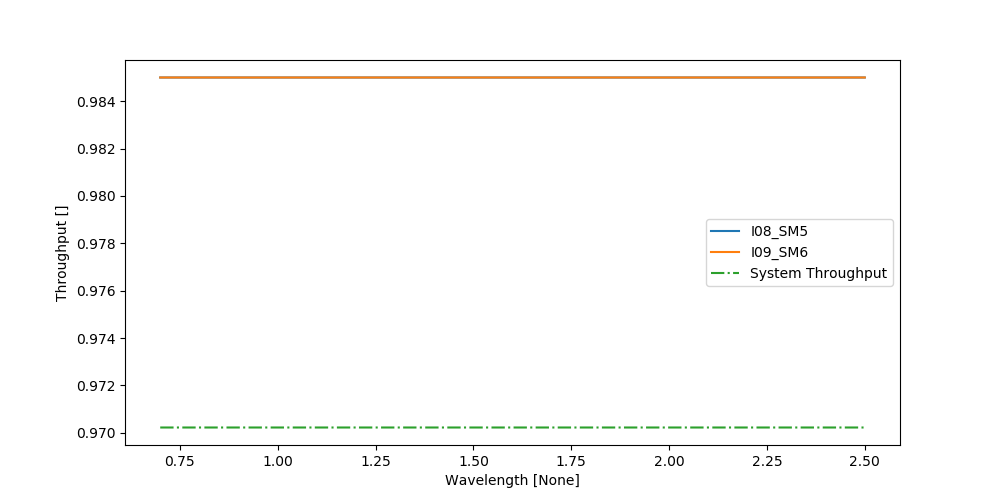
\includegraphics{micado_wide_field_mirror_list.png}}\phantomsection\label{fig-micado-wide-field-mirror-list}
\end{figure}

\setlength{\DUtablewidth}{\linewidth}
\begin{longtable*}[c]{|p{0.098\DUtablewidth}|p{0.075\DUtablewidth}|p{0.075\DUtablewidth}|p{0.075\DUtablewidth}|p{0.145\DUtablewidth}|p{0.133\DUtablewidth}|p{0.238\DUtablewidth}|}
\hline
\textbf{%
name
} & \textbf{%
outer
} & \textbf{%
inner
} & \textbf{%
angle
} & \textbf{%
temperature
} & \textbf{%
action
} & \textbf{%
filename
} \\
\hline
\endfirsthead
\hline
\textbf{%
name
} & \textbf{%
outer
} & \textbf{%
inner
} & \textbf{%
angle
} & \textbf{%
temperature
} & \textbf{%
action
} & \textbf{%
filename
} \\
\hline
\endhead
\multicolumn{7}{c}{\hfill ... continued on next page} \\
\endfoot
\endlastfoot

I08\_SM5
 & 
0.2
 & 
0.0
 & 
0
 & 
-190
 & 
reflection
 & 
TER\_mirror\_gold.dat
 \\
\hline

I09\_SM6
 & 
0.2
 & 
0.0
 & 
0
 & 
-190
 & 
reflection
 & 
TER\_mirror\_gold.dat
 \\
\hline
\end{longtable*}
\label{tbl-micado-wide-field-mirror-list}

The list of surfaces from the rotating optics wheel that are added to the optical train when observing in the wide field mode


\paragraph{Meta-data%
  \label{meta-data}%
}

\begin{quote}
\begin{alltt}
\begin{lstlisting}[frame=single]
            filename : LIST_MICADO_mirrors_wide.dat
                name : micado_wide_field_mirror_list
         pixel_scale : 0.004
         plate_scale : 0.26666666666
        element_name : MICADO_IMG_LR
              author : Kieran Leschinski
              source : Ric's SPIE 2018 PPT presentation
        date_created : 2018-11-19
       date_modified : 2019-07-10
              status : Design, pre PDR list of MICADO mirrors for wide-field mode
                type : mirror:list
          outer_unit : m
          inner_unit : m
          angle_unit : degree
    temperature_unit : deg_C
             z_order : [20, 120, 520]
             include : True
        ignore_wings : False
            wave_min : !SIM.spectral.wave_min
            wave_max : !SIM.spectral.wave_max
           wave_unit : !SIM.spectral.wave_unit
            wave_bin : !SIM.spectral.spectral_resolution
 report_plot_include : True
report_table_include : True
  minimum_throughput : !SIM.spectral.minimum_throughput
             etendue : !TEL.etendue
\end{lstlisting}
\end{alltt}
\end{quote}


\subsubsection{AtmosphericDispersionCorrection: \textquotedbl{}micado\_adc\_3D\_shift\textquotedbl{}%
  \label{atmosphericdispersioncorrection-micado-adc-3d-shift}%
}

\textbf{Included by default}: \texttt{False}

\textbf{File Description}: atmospheric disperson corrector

\textbf{Class Description}: <no docstring>

\textbf{Changes}:

\begin{itemize}
\item \end{itemize}


\paragraph{Data%
  \label{id1}%
}


\paragraph{Meta-data%
  \label{id2}%
}

\begin{quote}
\begin{alltt}
\begin{lstlisting}[frame=single]
            filename : None
                name : micado_adc_3D_shift
             include : False
         pixel_scale : 0.004
         plate_scale : 0.26666666666
        element_name : MICADO_IMG_LR
            altitude : !ATMO.altitude
           longitude : !ATMO.longitude
            latitude : !ATMO.latitude
             airmass : !OBS.airmass
         temperature : !ATMO.temperature
            humidity : !ATMO.humidity
            pressure : !ATMO.pressure
         pupil_angle : !OBS.pupil_angle
          efficiency : 1
            wave_mid : !SIM.spectral.wave_mid
           quick_adc : True
             z_order : [632, 232]
 report_plot_include : True
report_table_include : False
\end{lstlisting}
\end{alltt}
\end{quote}
